\section{Introduction}
% in recent years, the field of deep learning has seen a shift from uni modal learning towards multi modal learning.
The availability of multiple data types provides a rich source of information and holds promise for learning representations that generalise well across multiple modalities \parencite{baltrusaitis_multimodal_2019}.
Similar to how humans learn and extract information from their surrounding using their five senses, a machine learning model could learn from multiple data types.
Multimodal data naturally grants additional self-supervision in the form of shared information connecting the different data types.
However, the understanding of different modalities and the interplay between data types are non-trivial research questions and longstanding goals in machine learning research.
While fully-supervised approaches have been applied successfully \parencite{karpathy_deep_2015,tsai_learning_2018}, the labeling of multiple data types remains time-consuming and expensive.
Therefore, models that efficiently learn from multiple data types in a self-supervised fashion are much more widely applicable for real world problems.
%Therefore, it requires models that efficiently learn from multiple data types in a self-supervised fashion.
Learning the joint distribution of multiple data types without supervision can be done with self-supervised, generative models.

Here, we focus on variational autoencoders (VAEs) \parencite{kingma_auto-encoding_2014,rezende_stochastic_2014} which are able to jointly infer representations and generate new observations.
Despite their success on unimodal datasets, there are additional challenges associated with multimodal data \parencite{suzuki_joint_2016, vedantam_generative_2018}.
In particular, multimodal generative models need to represent both modality-specific and shared factors and generate semantically coherent samples across modalities.
Semantically coherent samples are connected by the information which is shared between data types \parencite{shi_variational_2019}.
These requirements are not inherent to the objective: the evidence lower bound (ELBO) of uni-modal VAEs.
Hence, adaptions to the original formulation are required to cater to and benefit from multiple data types.

% todo say that here we want to explore ways to make the joint distribution more flexible (by imporving the merging of unimoda distrs or by transforming the joint distribution with a flow)
% want to evaluate if we can achieve a more meaningfull, expressive latent representation with the f-mean (can be evaluated with the separability of the latent representation, the generation coherence (especially for missing modalities, where the mopoe method struggles the most).
% also want to give overview of hyperparameters and their influence

% motivation
A model that can generate any of the learned modalities, given any subset of modalities could be used for tasks where the model needs to translate from one modality to another for example, like image captioning.
It can also find applications in the medical domain, where the model could generate, given images and medical data of a patient, a text describing the medical condition of a patient.
Self-supervised training paradigms are especially usefull in the medical domain since there labeled data is expensive to acquire and thus very scarce.
% examples: (\citep{dorent_hetero-modal_2019}, \citep{calixto_latent_2019})


VAEs consist of two parts: an encoder part which maps the input data to a probability distribution and a decoder which learns to reconstruct the input from samples out of that latent distribution.
For $N$ modalities, $N$ different encoder and decoder pairs are needed, each encoder learning a unimodal latent distribution $q_n$.
To learn a joint distribution of multiple data modalities, some function $\mathcal{F}$ is needed that merges the information from all unimodal latent distributions into one joint distribution (see \cref{magic_graph}).


\begin{figure}
    \centering
    \label{magic_graph}
    \resizebox{0.9\textwidth}{!}{%
        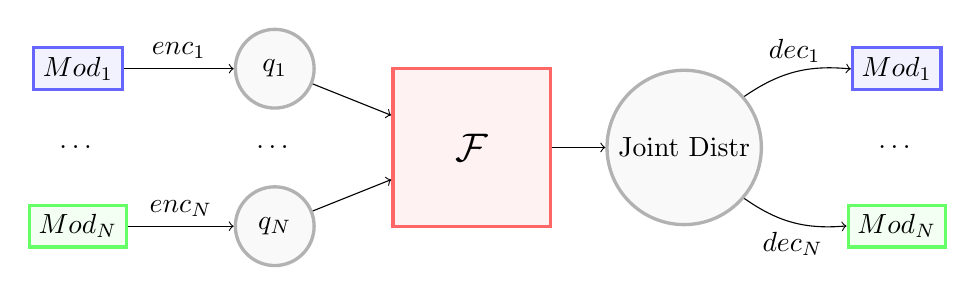
\begin{tikzpicture}[Mod1/.style={rectangle, draw=blue!60, fill=blue!5, very thick, minimum size=5mm},Mod2/.style={rectangle, draw=green!60, fill=green!5, very thick, minimum size=5mm},enc_mods/.style={circle, draw=gray!60, fill=gray!5, very thick, minimum size=10mm},magic/.style={rectangle, draw=red!60, fill=red!5, very thick, minimum size=20mm},]
            \node[Mod1] (mod1) {$Mod_1$};
            \node[below of=mod1] (points) {\ldots};
            \node[enc_mods, right of=mod1, xshift=1.5cm] (q1) {$q_1$};
            \node[Mod2, below of=points] (modn) {$Mod_N$};
            \node[enc_mods, right of=modn, xshift=1.5cm] (q2) {$q_N$};
            \node[below of=q1] (points) {\ldots};
            \node[magic, right of=q1, yshift=-1cm, xshift=1.5cm] (magic) {\Large$\mathcal{F}$};
            \node[enc_mods, right of=magic, xshift=1.7cm] (joint) {Joint Distr};
            \node[Mod1, right of=joint, xshift=1.7cm,yshift=+1cm] (rec_mod1) {$Mod_1$};
            \node[right of=joint,xshift=1.7cm] (points) {\ldots};
            \node[Mod2, right of=joint, xshift=1.7cm,yshift=-1cm] (rec_mod2) {$Mod_N$};
            \draw[->] (mod1) -- node[anchor=south] {$enc_1$} (q1);
            \draw[->] (q1) -- (magic);
            \draw[->] (modn) -- node[anchor=south] {$enc_N$} (q2);
            \draw[->] (q2) -- (magic);
            \draw[->] (magic) -- (joint);
            \draw[->] (joint) edge[bend left=20] node[anchor=south] {$dec_1$} (rec_mod1);
            \draw[->] (joint) edge[bend right=20] node[anchor=north] {$dec_N$} (rec_mod2);
        \end{tikzpicture}
    }
    \caption{\textbf{Flowchart depicting the main elements of a multi modal VAE wit $N$ different modalities.}
    Each input modality $n$ gets mapped to a unimodal latent distribution $q_n$ by an encoder $enc_n$.
    The $N$ unimodal learned distributions then get merged by a function $\mathcal{F}$ into a joint distribution from which the decoders can sample in order to reconstruct each of the $N$ modalities.}
\end{figure}

In previous work \parencite{wu_multimodal_2018,shi_variational_2019,sutter_generalized_2020}, learning a joint distribution has been done effectively by combining learned unimodal distributions with a geometric mean \parencite{wu_multimodal_2018}, an arithmetic mean \parencite{shi_variational_2019} or both \parencite{sutter_generalized_2020}.

%todo say that while both the MoE and PoE are sensible choices, there is no reason that they are the best -> would be better to have a merging function that is learnable by the model

Here, we generalize previous work by substituting $\mathcal{F}$ with a generalized $f$-Mean \parencite{niculescu_convex_2018}.
The generalized $f$-Mean being a generalisation of the arithmetic and the geometric mean, using it should bring results that are at least equally good or better than previous results if the objective is right.

The generalized $f$-Mean is defined as follows:
\begin{equation}
    \label{gfm}
    \mathcal{M}_{f}\left( \textbf{p} \right) = f^{-1}\left( \frac{1}{N} \sum ^N _{i=1} f(\textbf{p}_i)) \right)
\end{equation}

In \cref{gfm}, $f$ can be anything as long as it is invertible and differentiable, such that it can be parameterized as $f_{\psi}$ with trainable parameters $\psi$.
Normalizing Flows \parencite{papamakarios_normalizing_2019} present an approach to implement a sequence of invertible transformations with neural networks, such that they provide a natural implementation for $f_{\psi}$.

% todo maybe introduce notations:
%q for latent distributions
% M for number of modalities
% for iw samples K, index k
%  for index over subset: s, number of subsets: S
% index of samples of subsets:j (x_j \in X_s)

%todo summarize intro and work


% todo introduce that previous methods use the geometric or the arithmetic mean and that we are generalizing this here


For this project, I propose to use normalizing flows as a parameterisable function $f_\psi$ which combines the latent variables of multiple data types.
Normalizing flows are optimal for this task since they can transform simple initial densities into arbitrarily complex ones and vice versa.

Normalizing flows became very popular in the past years, and many methods already exist for different applications, however they have not yet been used to create a joint latent representation from multiple data types for VAEs.
The task in this project is to find an adequate implementation of normalizing flows, i.e. the best trade-off between the complexity of the resulting joint latent representation and the computational feasibility, and evaluate it on existing multimodal datasets.
To this end, I would first compare simpler methods, with a less good approximation of the true joint posterior but less computationally expensive, with more complex methods on toy datasets.
The ultimate goal being to construct a method that can learn a separable \footnote{separable in the sense that the joint latent representation can be separated into the different classes that span the dataset} joint latent representation from which coherent \footnote{coherent in the sense that all generated samples belong to the same class} samples can be generated on the challenging MIMIC-CXR \parencite{johnson_mimic-cxr-jpg_2019} database.